\documentclass{beamer}

\usetheme{Madrid}

\usepackage[utf8]{inputenc}
\usepackage[T1]{fontenc}
\usepackage{float}
\usepackage{listings}
\usepackage{amsmath}
\usepackage{amssymb}
\usepackage[mathcal]{euscript}

\title[The BLS Signature Scheme]{The BLS Signature Scheme}
\author[Gabor Tanz]{Gabor Tanz}
\institute[BFH]{Berne University of Applied Sciences}
\date[2019]{2019}

\AtBeginSection[]
{
	\begin{frame}
		\frametitle{Table of Contents}
		\tableofcontents[currentsection]
	\end{frame}
}

\begin{document}

\frame\titlepage

\begin{frame}
	\frametitle{Table of Contents}
	\tableofcontents
\end{frame}

\section{Introduction}
\begin{frame}{Introduction}
	What is BLS?
	\begin{itemize}
		\item Signature method based on bilinear pairing in an EC group
		\item Invented by Boneh, Lynn and Shacham
		\item Uses Weil pairing
		\item Has short signatures
		\item And more (later)
	\end{itemize}
\end{frame}
\section{Prerequisites}
\subsection{Abstract algebra}
\begin{frame}{Abstract algebra}
	Groups
	\begin{itemize}
		\item Set with binary operation, inverse and identity
		\item Operation produces another element of group
		\item Mathematical definition: $\mathcal{G} = (G, \circ, inv, e)$
		\item Order of group $ord$-> number of elements
		\item Ex: the set of integers $\mathbb{Z}$ modulo $n$ with the operation $\times$, the identity element 1 and the inverse operation $^{-1}$. $\mathcal{G} = (\mathbb{Z}_{n}^*, \times, ^{-1}, 1)$
	\end{itemize}
\end{frame}
\begin{frame}{Abstract algebra}
	Cyclic Groups
	\begin{itemize}
		\item Group can be generated by $x$
		\item Usually group mod $n$
		\item $ord(x)$ must be $ord(\mathcal{G})$
		\item Ex: 3 is a generator of $\mathbb{Z}_7^*$. The powers of 3 mod 7 are 3,2,6,4,5,1, which are all elements in $\mathbb{Z}_7$.
	\end{itemize}
\end{frame}
\begin{frame}{Abstract algebra}
	Fields
	\begin{itemize}
		\item set with two operations $(K, +, *)$
		\item based on two groups $(K, +, -, 0)$ and $(K, *, ^-1, 1)$
		\item groups are distributive
		\item Ex: $(\mathbb{Z}$ mod 5 $, +, -, 0, *, ^{-1}, 1)$, which consists of the groups $(\mathbb{Z}$ mod 5 $, +, -, 0)$ and $(\mathbb{Z}$ mod 5 $, *, ^{-1}, 1)$.
	\end{itemize}
\end{frame}
\subsection{Elliptic curves}
\begin{frame}{Elliptic curves}
	Basics
	\begin{itemize}
		\item Set of points satisfying $y^2 = x^3 + ax + b$
		\item Defined over $\mathbb{F} = (F, +, -, 0, *, ^{-1}, 1)$
	\end{itemize}
	\begin{figure}[hbt!]
		\centering
		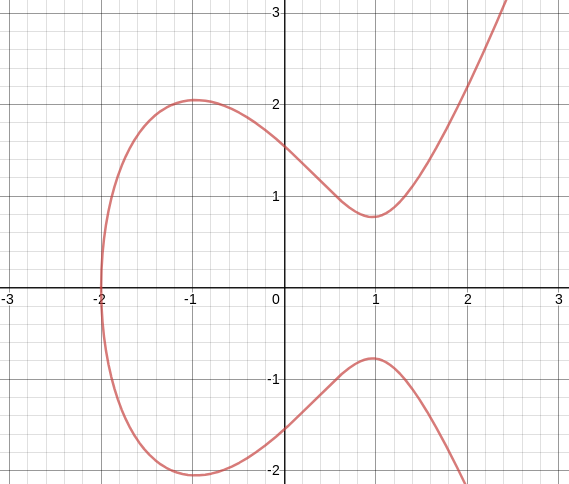
\includegraphics[width=0.5\linewidth]{ec1}
		\caption[]{Example of an elliptic curve: $y^2 = x^3 - 2.8x + 2.4$}
		\label{fig:ec-b2}
	\end{figure}
\end{frame}
\begin{frame}{Elliptic curves}
	Addition of points
	\begin{itemize}
		\item intersection always at 3 points (tangential counts twice)
		\item addition of $P$ and $Q$ is mirror of 3rd intersection
	\end{itemize}
	\begin{figure}[hb!]
		\centering
		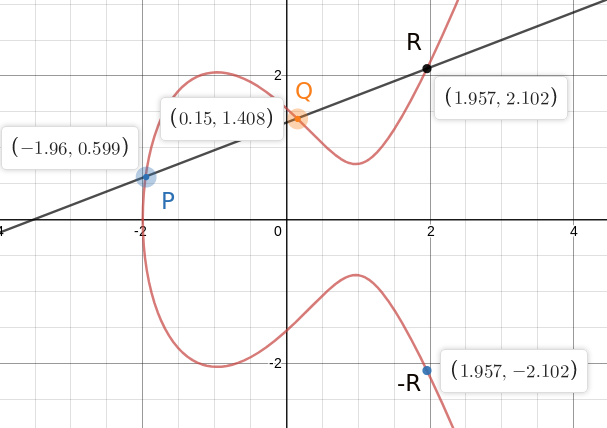
\includegraphics[width=0.5\linewidth]{ec2}
		\caption[]{Example with $P, Q, R$ and $-R$}
	\end{figure}
\end{frame}
\begin{frame}{Elliptic curves}
	EC over finite Fields
	\begin{itemize}
		\item Field given by $(\mathbb{Z}_p,+,-,0,\times,^{-1},1)$ if $p$ with $p$ being prime
		\item Points repeat (wraparound)
	\end{itemize}
	\begin{figure}[hbt!]
		\centering
		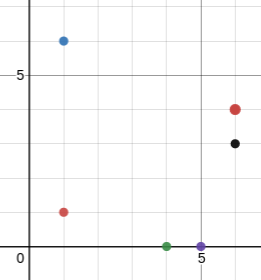
\includegraphics[width=0.4\linewidth]{ec3}
		\caption{$y^2 \equiv x^3 + 2x + 5$ mod $7$}
	\end{figure}
\end{frame}
\subsection{Bilinear maps}
\begin{frame}{Bilinear maps}
	\begin{itemize}
		\item Maps two additive groups $G$ of $ord(p)$ to multiplicative target Group $G_t$ $e: G_1 \times G_2 \rightarrow G_t$
		\item commutativity for additive and multiplicative operations
		\item distributivity for multiplicative operations
		\item $e(u^a,v^b) = e(u^b,v^a)$ as $e(u,v)^{ab} = e(u,v)^{ba}$ or $e(a\times{u},b\times{v}) = e(u,ab\times{v}) = e(ab\times{u},v) = e(u,v)^{ab}$
	\end{itemize}
	\begin{figure}[hbt!]
		\centering
		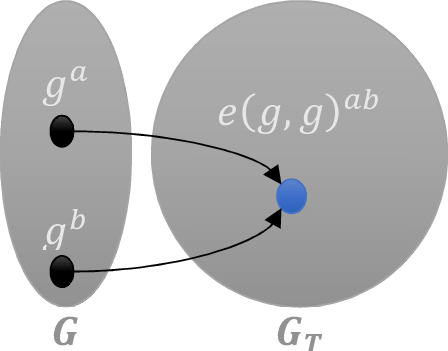
\includegraphics[width=0.25\linewidth]{pairing1}
		\caption{illustration of pairing}
	\end{figure}
\end{frame}
\section{Signature schemes}
\subsection{Key generation}
\begin{frame}{Key generation}
	content...
\end{frame}
\subsection{Signature generation}
\begin{frame}{Signature generation}
	content...
\end{frame}
\subsection{Signature validation}
\begin{frame}{Signature validation}
	content...
\end{frame}
\subsection{Hash functions}
\begin{frame}{Hash functions}
	content...
\end{frame}
\section{BLS signatures}
\begin{frame}{BLS signatures}
	content...
\end{frame}
\subsection{Signature aggregation}
\begin{frame}{Signature aggregation}
	content...
\end{frame}
\subsection{Threshold signatures}
\begin{frame}{Threshold signatures}
	content...
\end{frame}
\section{Usage of BLS for cryptocurrencies}
\begin{frame}{Splitting of private key}
	content...
\end{frame}
\begin{frame}{Multiparty signatures}
	content...
\end{frame}
\begin{frame}{Signature aggreation of transaction blocks}
	content...
\end{frame}
\section{Conclusion}
\begin{frame}{Conclusion}
	content...
\end{frame}

\end{document}